\section{Architecture Integration}

\subsection{Model Support}

\begin{table}[H]
\centering
\small
\begin{tabular}{lllll}
\toprule
\textbf{Model} & \textbf{Attention class} & \textbf{Nested?} & \textbf{RoPE?} & \textbf{GQA?} \\
\midrule
DistilBERT & \texttt{MultiHeadSelfAttention} & No & No & No \\
RoBERTa & \texttt{BertSelfAttention} (nested) & Yes & No & No \\
GPT-2 & \texttt{GPT2Attention} (Conv1D) & No & No & No \\
Qwen3.5 & \texttt{Qwen3Attention} & No & Yes & Yes \\
\bottomrule
\end{tabular}
\end{table}

\subsection{Weight Extraction}

MinimalAURORA uses a \textbf{layered extraction strategy}:

\subsubsection{Priority Order}

\begin{enumerate}
\item \textbf{UniversalAdapter} -- tried first, covers many cases.
\item \textbf{GPT-2 fused \texttt{c\_attn}} -- transpose and split.
\item \textbf{RoBERTa nested \texttt{self.query/key/value}} -- extract from inner block.
\item \textbf{Named mappings} -- \texttt{q\_proj}, \texttt{q\_lin}, \texttt{query}, etc.

\end{enumerate}
\subsubsection{GPT-2 Conv1D Handling}

\begin{lstlisting}
if ("Conv1D" in p\_cls or hasattr(base\_c, "nf")
    or (weight.dim() == 2 and weight.shape[1] == 3 * self.hidden\_size)):
    weight = weight.t()
\end{lstlisting}

The heuristic \texttt{weight.shape[1] == 3 * hidden} catches the case where 
Conv1D stores weights as \texttt{(in, 3*out)}.

\subsubsection{RoBERTa Nested Detection}

Detection logic:

\begin{lstlisting}
if hasattr(src, "self") and hasattr(src.self, "query"):
    is\_nested = True
elif (cls\_name in ("BertSelfAttention", "RobertaSelfAttention", ...)
      or (cls\_name.endswith("SelfAttention") and not has\_out\_proj)):
    is\_nested = True
self.is\_nested\_encoder = is\_nested
\end{lstlisting}

For DistilBERT: \texttt{MultiHeadSelfAttention} ends with "SelfAttention" but 
has \texttt{out\_lin} $\to$ NOT nested. Good.

For RoBERTa: \texttt{BertAttention} has \texttt{self} and \texttt{output} $\to$ nested. Good.

\subsubsection{Nested Encoder Output Projection}

For nested encoders, the output projection is set to \textbf{identity}:

\begin{lstlisting}
elif proj\_key == "o" and self.is\_nested\_encoder:
    eye\_w = torch.eye(self.hidden\_size, self.all\_head\_size)
    target.decompose\_from\_weight(eye\_w, None, self.energy)
\end{lstlisting}

And in forward:

\begin{lstlisting}
if self.is\_nested\_encoder:
    output = context * self.output\_scale
else:
    output = self.out\_proj(context) * self.output\_scale
\end{lstlisting}

\subsection{Injection}

\begin{lstlisting}
def inject\_minimal\_aurora(layer, model\_config, old\_attn=None, **kwargs):
    new\_attn = MinimalAURORAAttention(model\_config=model\_config, ...)
    
    src\_attn = old\_attn or find\_attention(layer)
    if src\_attn is not None:
        try:
            new\_attn.copy\_weights(src\_attn)
        except Exception as e:
            logger.error(f"copy\_weights failed: {e}")
            return None  # silent failure
        # transfer device/dtype
        p = next(src\_attn.parameters())
        new\_attn.to(device=p.device, dtype=p.dtype)
    
    # replace attention
    if hasattr(layer, "attention"):
        if hasattr(layer.attention, "self"):
            layer.attention.self = new\_attn
            new\_attn.is\_nested\_encoder = True
        else:
            layer.attention = new\_attn
    elif hasattr(layer, "self"):
        layer.self = new\_attn
        new\_attn.is\_nested\_encoder = True
    
    return new\_attn
\end{lstlisting}

\textbf{Note.} The injection returns \texttt{None} on failure, which is \textbf{silent}. 
Unlike A3/AASVD (which raise), this requires the caller to check the 
return value.

\subsection{The `FactorisedLinear` Module}

\begin{lstlisting}
class FactorisedLinear(nn.Module):
    def \_\_init\_\_(self, in\_features, out\_features, rank=64, bias=True,
                 energy=0.95, lora\_rank=16, lora\_alpha=32.0):
        super().\_\_init\_\_()
        self.down = nn.Linear(in\_features, rank, bias=False)
        self.up = nn.Linear(rank, out\_features, bias=bias)
        
        if lora\_rank \textgreater{} 0:
            self.lora\_A = nn.Parameter(torch.randn(lora\_rank, in\_features) * 0.01)
            self.lora\_B = nn.Parameter(torch.zeros(out\_features, lora\_rank))
        
        self.reset\_parameters()
\end{lstlisting}

\subsection{The `output\_scale` Parameter}

\begin{lstlisting}
self.output\_scale = nn.Parameter(torch.ones(1))
\end{lstlisting}

Applied in forward:

\begin{lstlisting}
output = self.out\_proj(context) * self.output\_scale
\end{lstlisting}

This is a new parameter not present in the base checkpoint. It 
initializes to 1.0 and is trainable. During recovery training, it 
may drift. If it reaches 0, the entire attention output collapses.

\subsection{The `pres\_gate` Parameter (Unused)}

\begin{lstlisting}
self.pres\_gate = nn.Parameter(torch.tensor(2.0))
\end{lstlisting}

\textbf{This parameter is defined but never used in the forward pass.} It 
appears to be a leftover from a previous design (perhaps a preservation 
gate between attention output and residual). We document this in  8.6 
and recommend removal.

\subsection{Failure Modes}

\begin{table}[H]
\centering
\small
\begin{tabular}{ll}
\toprule
\textbf{Failure} & \textbf{Response} \\
\midrule
Missing projection & \texttt{copy\_weights} raises RuntimeError \\
Small Frobenius norm & Raises RuntimeError \\
Injection error & Returns None (silent) \\
\texttt{output\_scale} drift to 0 & Attention output collapses \\
\texttt{pres\_gate} unused & No effect \\
\bottomrule
\end{tabular}
\end{table}

\subsection{Registry}

\begin{lstlisting}
@ATTENTION\_REGISTRY.register("minimal\_aurora", supports\_causal=True, supports\_gqa=True)
class MinimalAURORAAttention(BaseAttention):
    ...
\end{lstlisting}

\subsection{Cross-Attention}

Forward accepts \texttt{encoder\_hidden\_states} and supports cross-attention 
(though GQA + cross-attention interaction may have edge cases).



\begin{figure}[H]
\centering
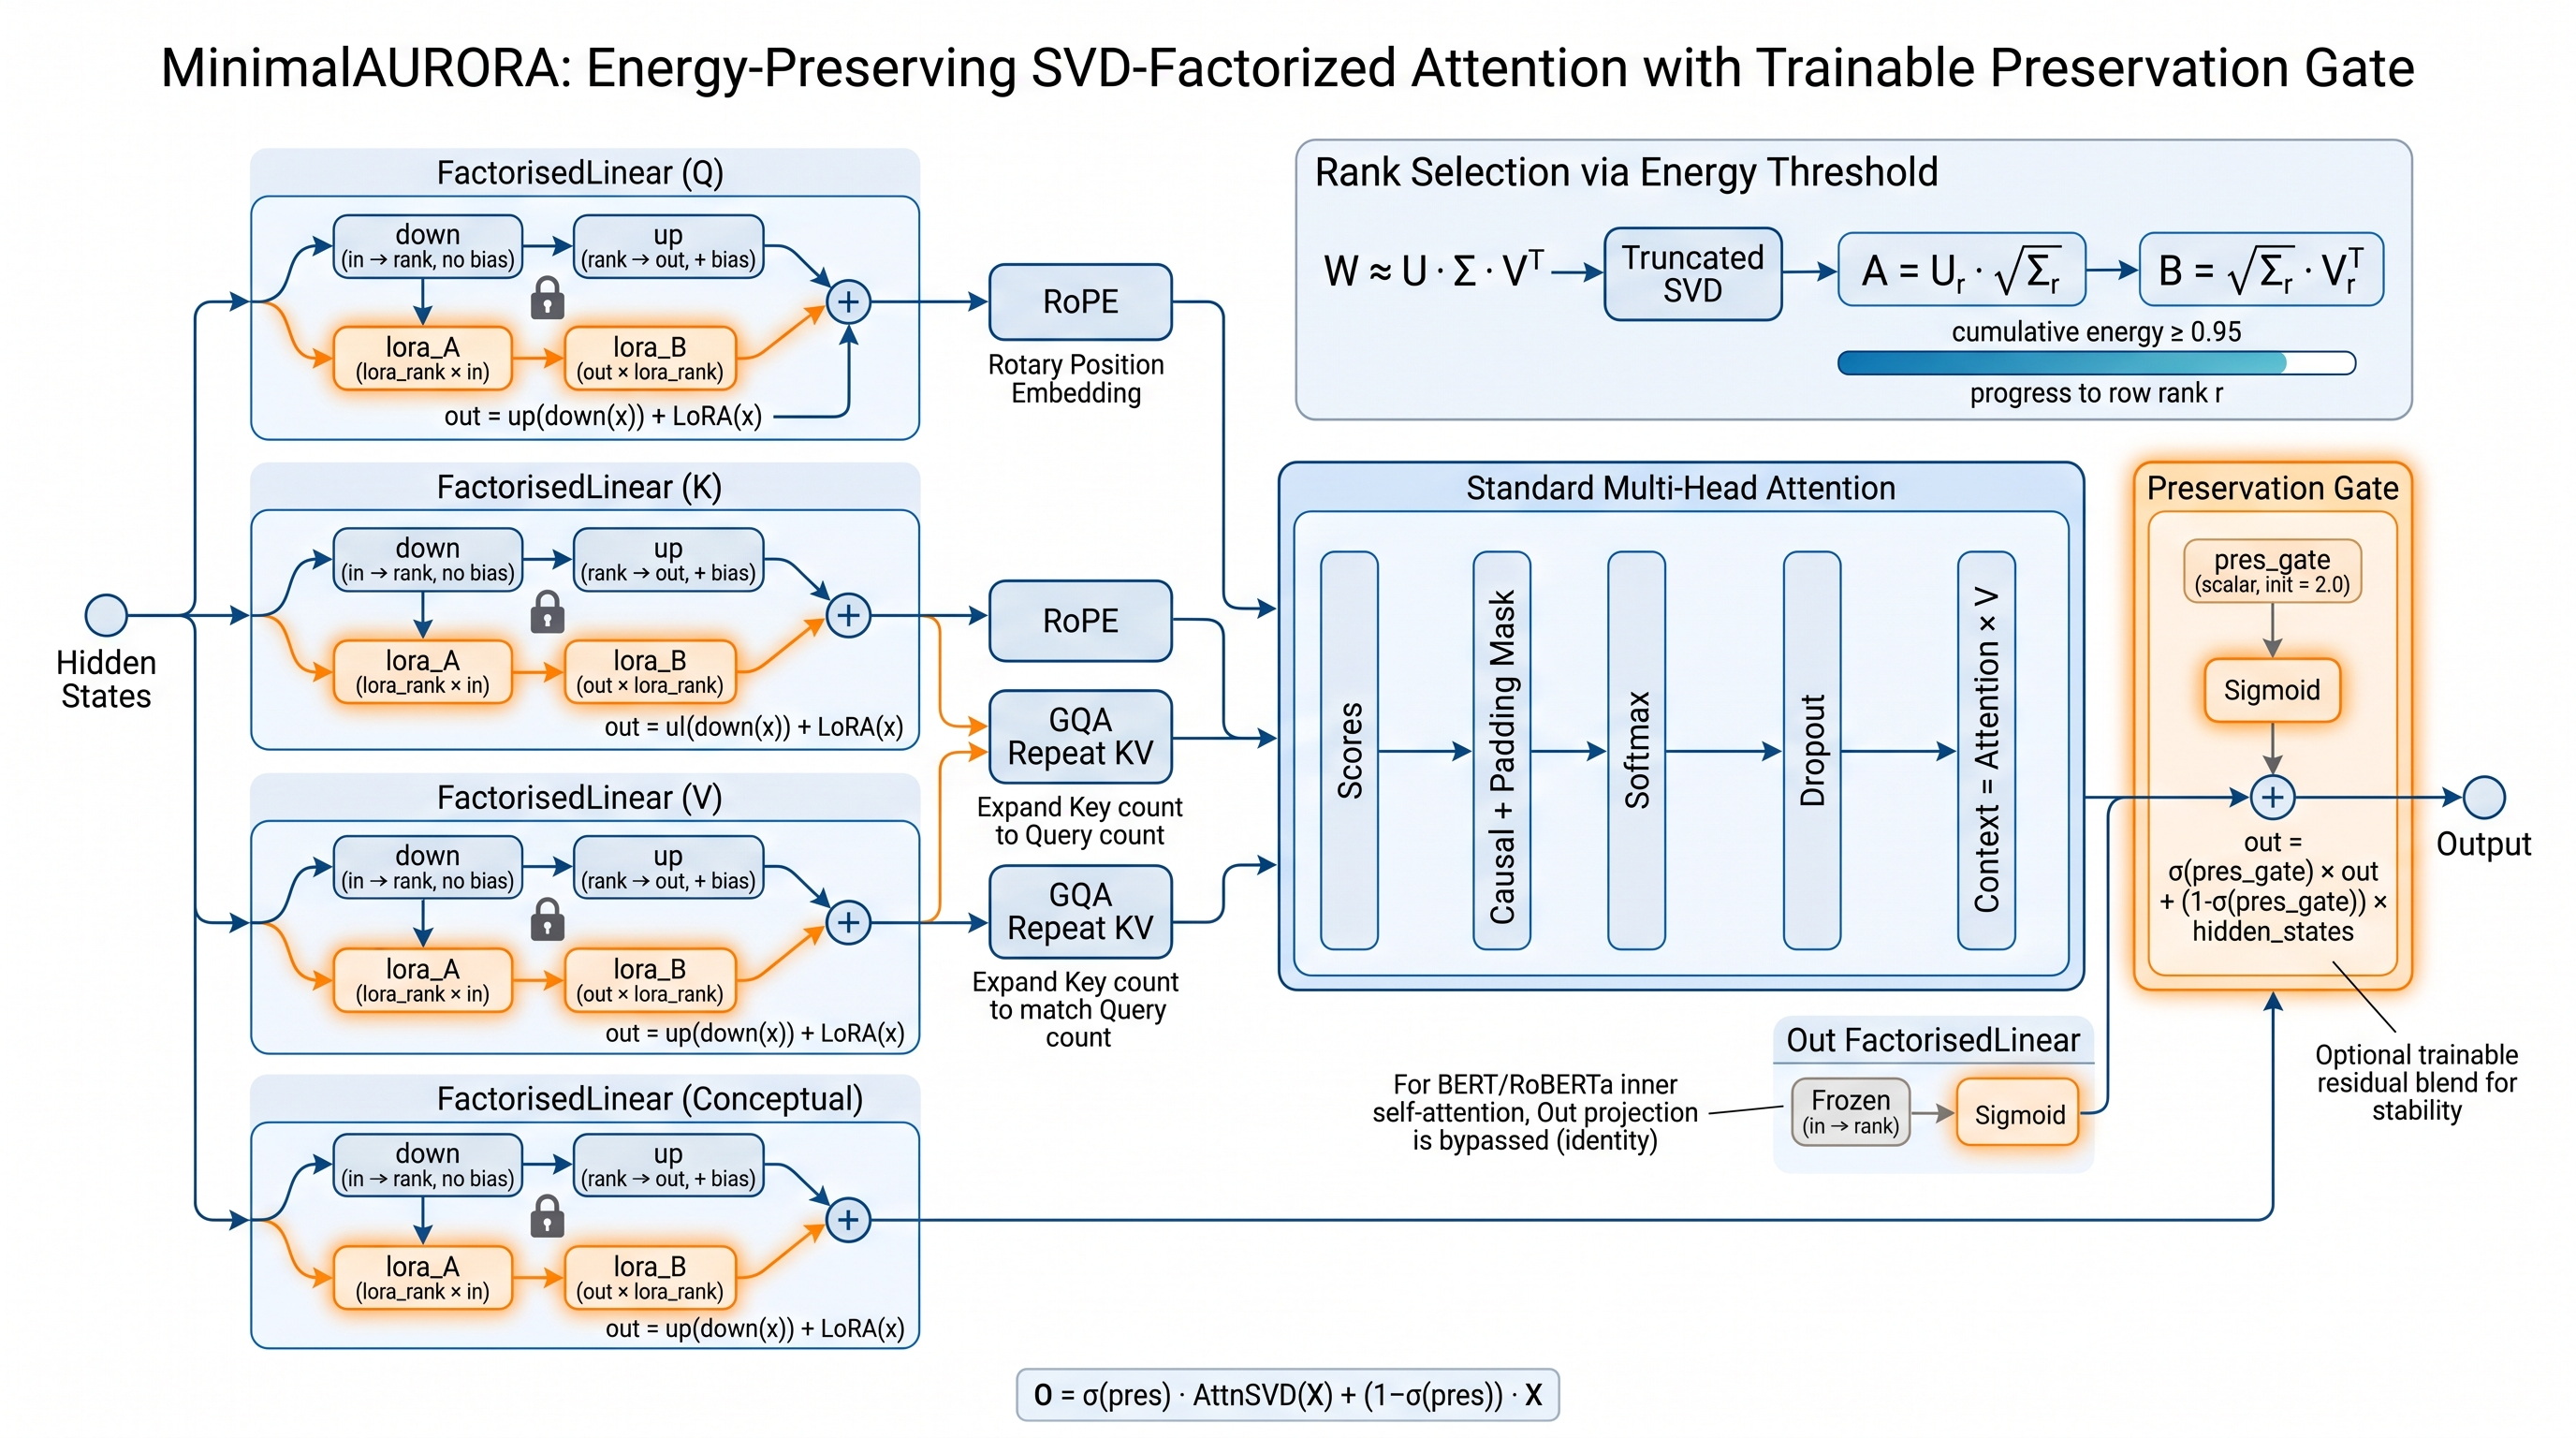
\includegraphics[width=\linewidth]{figures/architecture.jpeg}
\caption{High-level architectural diagram of minimal\_aurora.}
\label{fig:arch_minimal-aurora}
\end{figure}

